\section{Modelli per sistemi paralleli}
E' qualcosa di complesso che richiede una parte HW e software, bisogna necessariamente fare delle astrazioni perche' non ci potremo occupare di tutti i dettagli.
Abbiamo questa astrazione:
\begin{itemize}
    \item Livello macchina: assembly
    \item Modello architetturale: SIMD o MIMD, si prevedono anche processi in cui ci sono tante unita' di calcolo che interagiscono tra di loro, gestione multi processi e multi thread
    \item Modello computazionale: e' un modello formale che consente di descrivere la macchina astraendo dai modello sottostanti ed e' fondamentale per la creazione degli algoritmi. Processore, memoria, scambio dati con un BUS. E' inerentemente sequenziale ma e' utile per creare l'algoritmo data la size dei dati. Nell'ambito del parallelismo passiamo dal modello RAM al PRAM (modello RAM per architetture parallele)
    \item Modello di programmazione parallela: e' il modo con cui gestiamo il sistema di calcolo parallelo esprimendo algoritmi con un linguaggio che espone il prallelismo dell'architettura sottostante per essere eseuito da un linguaggio che ha in se elementi che permettono di usare il parallalismo. Vi sono aspetti di comunicazione per gestire il multi threading, si affronta quindi la suddivisione del compito in processi e thread. Fino ad arrivare a problemi legati all'uso o della gestione di spazi di indirizzamento condivisi.
\end{itemize}

\subsection{SIMD}
Si parla di unita' molteplici che lavorano sui dati, laddove i dati permettono di sviluppare meccanismi paralleli. E' un mondo vasto che si puo' vedere anche nelle architetture comuni dove si ha la divisione di computazione in diverse ALU specializzate, una che lavora su un singolo registro ed una che lavora vettorialmente ed e' quindi in grado di lavorare su piu' dati contemporaneamente. Nelle GPU parleremo di thread che lavorano simultaneamente in modalita' SIMD.

\subsection{MIMD}
E' un'altro dei modelli molto diffusi paralleli in cui si hanno le istruzioni di tanti dati simultaneamente che vengono eseguite da un numero di processori veramente grandi.

\subsection{PRAM}
Il modello PRAM e' il modello di calcolo parallelo piu' semplice, in questo caso abbiamo una memoria condivisa, i processori lavorano in maniera SIMD ovvero fanno la stessa istruzione, esistono anche processori inattivi.
Ci da quanti passi ci servono per risolvere l'algoritmo parallelo, anche in questo caso potremmo fare studio di complessita' per risolvere il problema parallelo.

\subsection{Parallelizzazione di algoritmi}
Quando vorremo vedere la complessita' computazionale degli algoritmi dovremo fare delle astrazioni ed usare qualcosa simile al PRAM.
Nella pratica si partira' da un algoritmo sequenziale, dovremo vedere come dividere la computazione in parallelo per capire come le varie parti vengano attribuite ai vari thread, tendenzialmente la partizione logica dei task la faremo noi, la parte dello scheduling se ne occupa il sistema ma e' bene conoscela perche' ad esempio in CUDA i processi di scheduling sono fortemente condizionanti dalla potenza del sistema e dovremo adeguare gli algoritmi sulla base dei meccanismi di scheduling. Quello che vorremo ottenere e' una massima occupancy delle unita' di calcolo.
Dipendentemente dal modello di memoria, un task può accedere a memoria condivisa o usare tecniche di message passing.

\section{CPU multi-core e programmazione multi-threading}
Un programma in esecuzione e' un processo che viene allocato nel OS e ha una serie di risorse che ha, convive con altri processi nel sistema ed e' una cosa abbastanza pesante, mentre i thread che compongono un processo sono dei sotto-processi ma piu' leggeri. Un processo in genere consiste di tanti thread. In genere vengono creati da delle operazioni di sistema come le fork in UNIX e vengono terminati dall'OS.
I processi hanno il loro contesto e vengono eseguit sequenzialmente secondo un flusso, anche i thread eseguono le cose sequenzialmente ma essendo molteplici possono essere parallali.
Il thread e' un singolo flusso di istruzione che si trova in un processo che lo scheduler si occupa di eseguire concorrentemente ad altri threads.

\subsection{Thread}
Ha un ciclo di vita, viene generato e viene ucciso, il processo chiude quando tutti i thread hanno terminato la loro esecuzione:
\begin{itemize}
    \item New: viene generato, chi lo ha generato sa chi e' 
    \item Executable: il thread e' pronto per essere eseguito quando ha tutte le risorse necessarie
    \item Running: il thread sta attualmente eseguendo le sue istruzioni
    \item Waiting: il thread sta aspettando che una risorsa diventi disponibile
    \item Finished: il thread ha completato la sua esecuzione e viene rimosso
\end{itemize}

\begin{figure}[ht!]
    \centering
    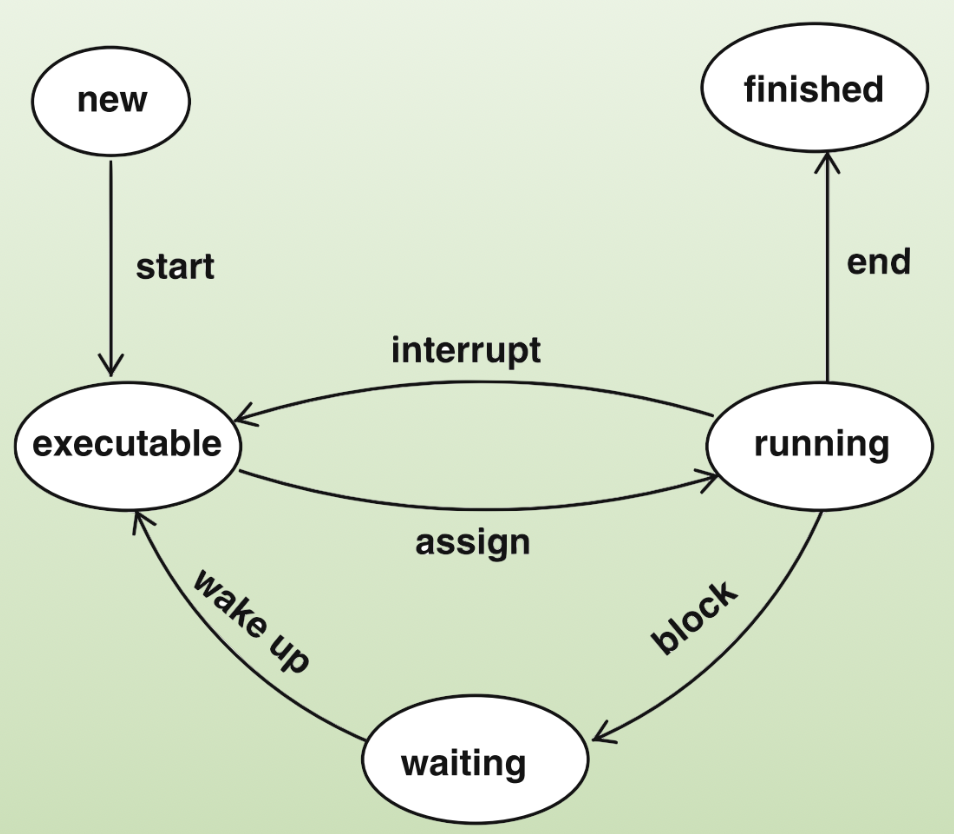
\includegraphics[width=0.5\textwidth]{images/statiThread.png}
    \caption{Stati di un thread}
\end{figure}

I vantaggi sono:
\begin{itemize}
    \item Si possono avere tanti flussi di esecuzioni che possono avvantaggiarsi di sistemi multi-core
    \item Visibilita' dei dati globale
    \item Semplicita' di gestione eventi asincroni come l'io 
    \item Velocita' di context switching
\end{itemize}

Le difficolta' sono la concorrenza e il problema di avere uno spazio privato.

\section{Programmazione multi-core}
Noi vedremo la programmazione multi-thread su architetture multi-core. L'applicazione deve essere progettata considerando diversi fattori del sistema di calcolo parallelo multi-core (e many core come le GPU), bisogna trovare di task, bilanciarli, suddividere i dati sui vari task (il problema e i dati lo devono consentire) e farlo in modo che tutti i task possano lavorare su queste porzioni di dati indipendentemente. Ci sono quindi tanti aspetti da tenere in considerazione sulla dipendenza e indipendenza dei dati. Test e debugging sono anchessi importanti quando si sviluppano gli algoritmi in ambito parallelo perche' ci sono tanti flussi di esecuzione.

\section{Programmazione CUDA}
Pensare in parallelo significa avere chiaro quali feature la GPU espone al programmatore. Si lavora come su pthread o OpenMP. Si scrive una porzione di CUDA C (semplice estensione di C) per l'esecuzione sequenziale e lo si estende a migliaia di thread (permette di pensare 'ancora' in sequenziale)

\begin{itemize}
    \item I dati stanno su host
    \item allocare spazio su GPU
    \item copiare i dati da host a GPU
    \item allocare memoria per l'output
    \item lanciare il kernel che elabora dati in ingresso e li mette in output, mette una copia su memoria condivisa
    \item cancellare le memorie allocate
\end{itemize}

\subsection{Organizzazione dei thread}
Cuda presenta una gerarchia astratta di thread che si distribuisce su due livelli:
\begin{itemize}
    \item grid: una griglia ordinata di blocchi
    \item block: un insieme di thread che possono cooperare tra loro
\end{itemize}
Questi possono avere dimensioni 1D, 2D o 3D. Tutto questo fa 9 combinazioni tra grid e block.

\begin{figure}[ht!]
    \centering
    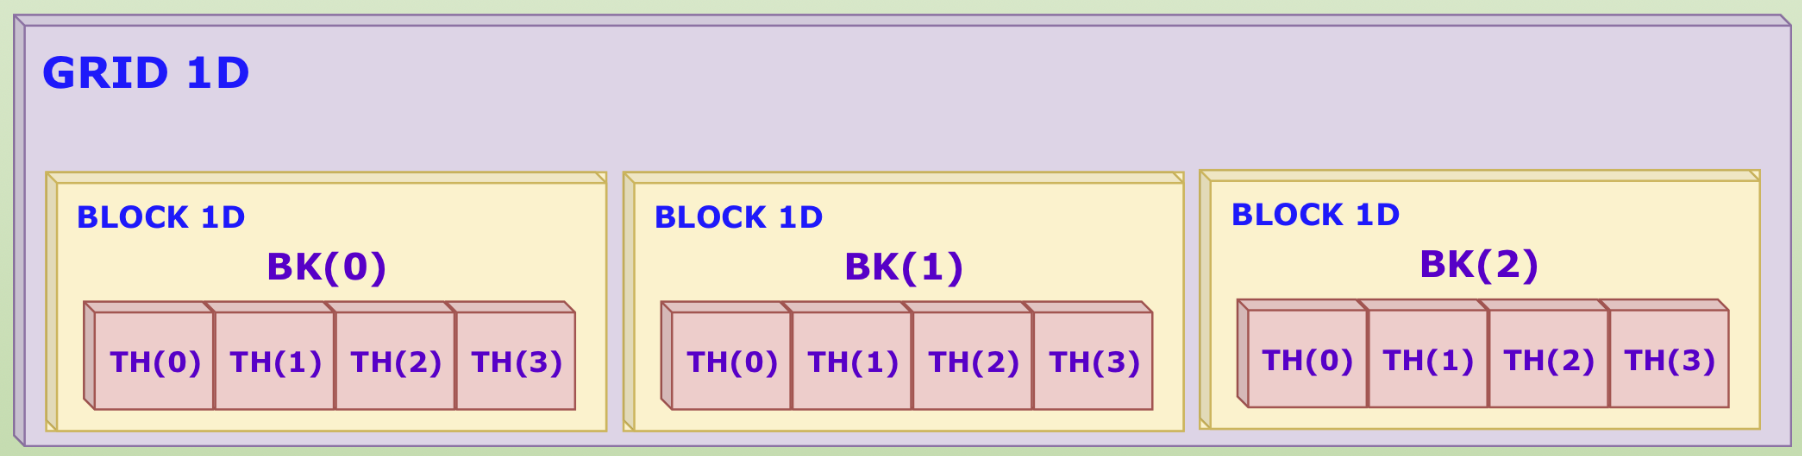
\includegraphics[width=0.5\textwidth]{images/organizzazioneThread.png}
    \caption{Organizzazione dei thread in CUDA}
\end{figure}

Ci sono delle limitazioni, un blocco puo' contenere al massimo 1024 thread.

Il blocco di thread e' molto importante, dal punto di vista semantico ha un significato, e' un gruppo di thread che possono cooperare tra loro tramite:
\begin{itemize}
    \item block-local synchronization, sincronizzazione: cooperare per uno stesso compito avvantaggiandosi da operazioni fatte da altri thread
    \item block-local communication, comunicazione tramite la shared memory: e' una memoria cache che quindi ha tempi di accesso di molto ridotti
\end{itemize}

I thread vengono identificati univocamente tramite l'id di blocco e l'id di thread. blockIdx e threadIdx sono specificati in variabili globali, un kernel a runtime ha accesso a queste informazioni che vengono assegnate dinamicamente, hanno tre valori x, y, z di tipo uint32.

\begin{lstlisting}[language=C]
    
#include <stdio.h>

__global__ void checkIndex(void) {
	printf("threadIdx:(%d, %d, %d) blockIdx:(%d, %d, %d) "
					"blockDim:(%d, %d, %d) gridDim:(%d, %d, %d)\n",
					threadIdx.x, threadIdx.y, threadIdx.z,
					blockIdx.x, blockIdx.y, blockIdx.z,
					blockDim.x, blockDim.y, blockDim.z,
					gridDim.x,gridDim.y,gridDim.z);
}

/*
* MAIN
*/
int main(int argc, char **argv) {

	// grid and block definition
	dim3 block(4);
	dim3 grid(3);

	// Print from host
	printf("Print from host:\n");
	printf("grid.x = %d\t grid.y = %d\t grid.z = %d\n", grid.x, grid.y, grid.z);
	printf("block.x = %d\t block.y = %d\t block.z %d\n\n", block.x, block.y, block.z);

	// Print from device
	printf("Print from device:\n");
	checkIndex<<<grid, block>>>();

	// reset device
	cudaDeviceReset();
	return(0);
}
\end{lstlisting}
Abbiamo accesso alle dimensioni della griglia e del blocco tramite le variabili blockDim e gridDim, che sono anchessi di tipo uint32. Anche in questo caso abbiamo tre componenti x, y, z.

L'indice univoco del thread nei blocchi si calcola differentemente rispetto alle dimensioni del blocco:

\begin{figure}[ht!]
    \centering
    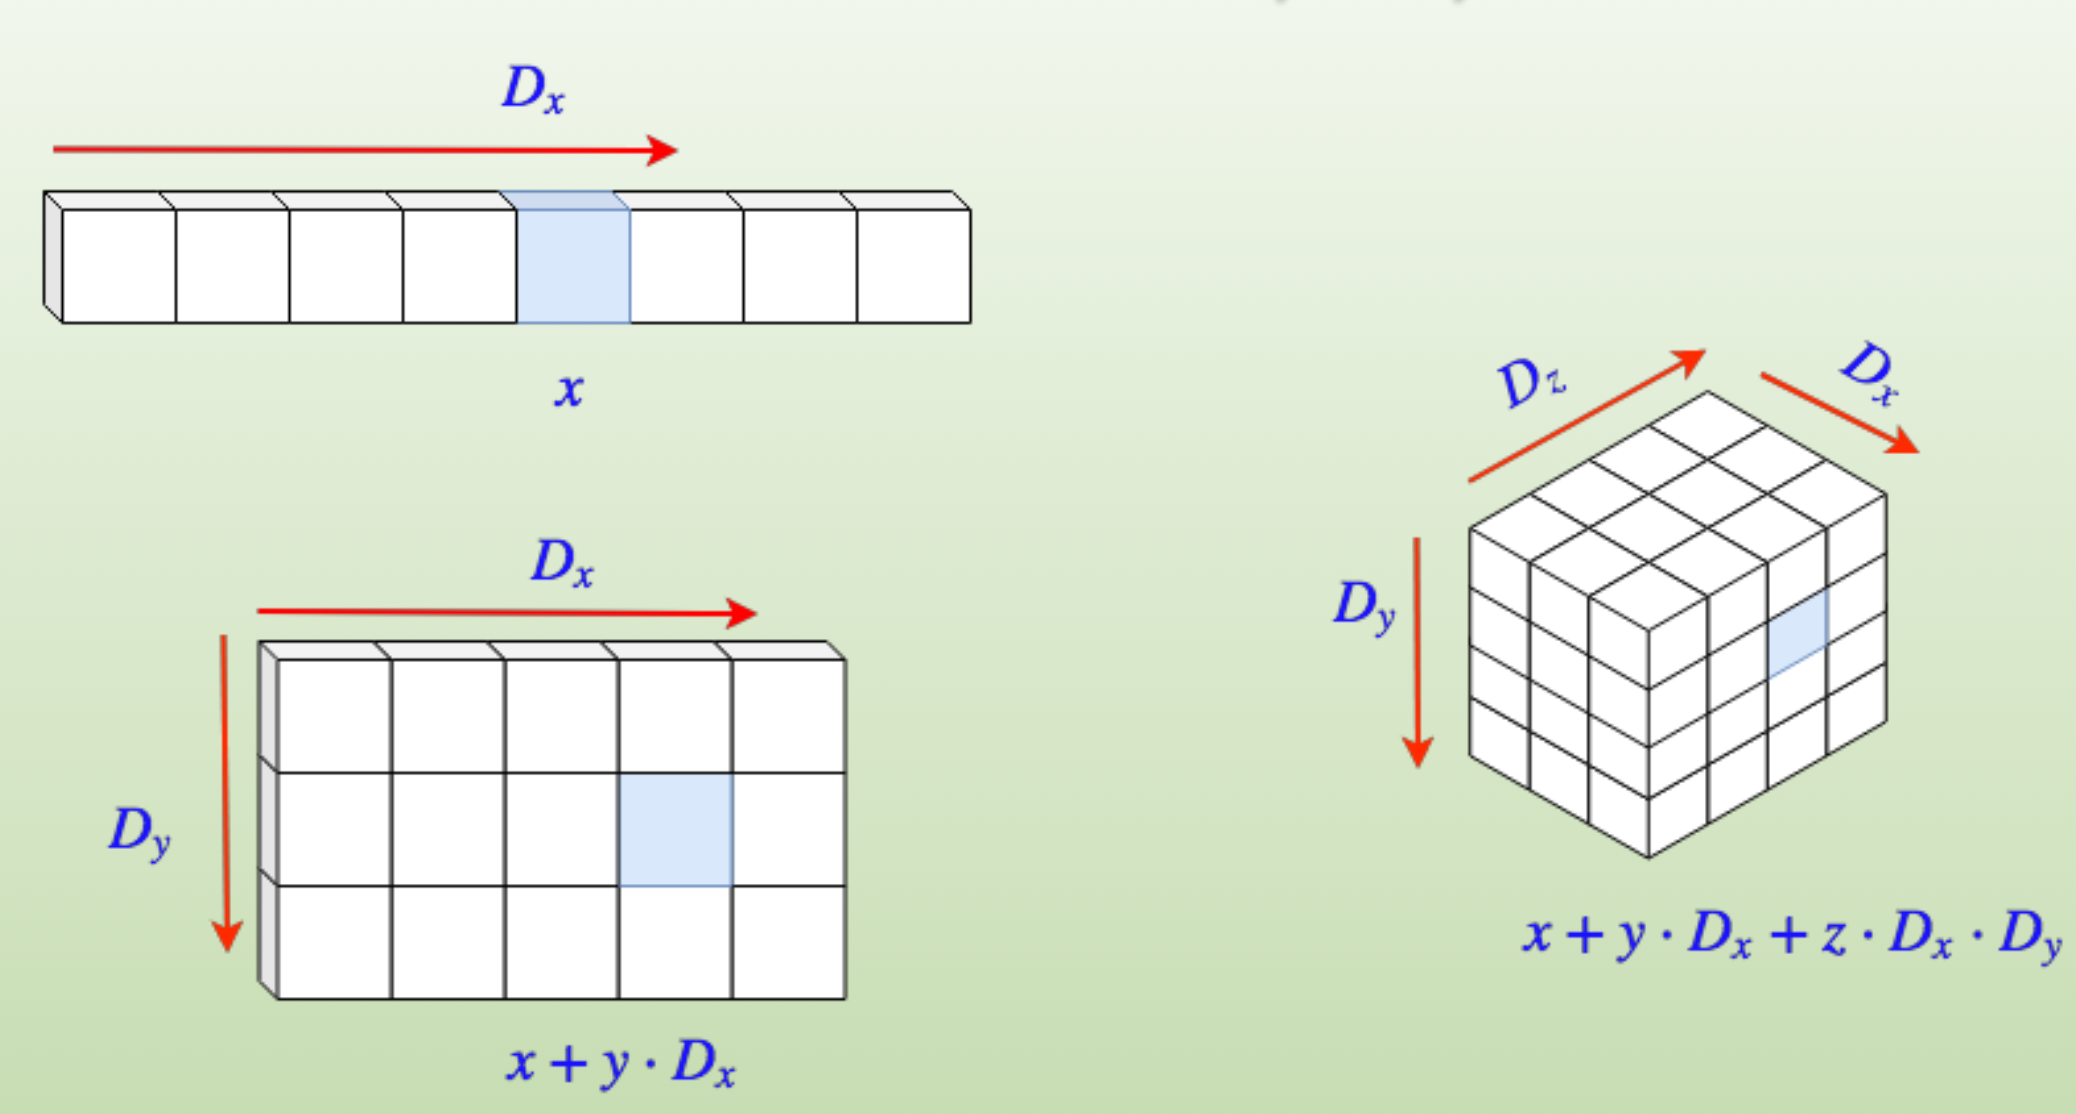
\includegraphics[width=0.8\textwidth]{images/indiceUnicoBlocchi.png}
    \caption{Indice univoco dei thread nei blocchi}
\end{figure}


\begin{figure}[ht!]
    \centering
    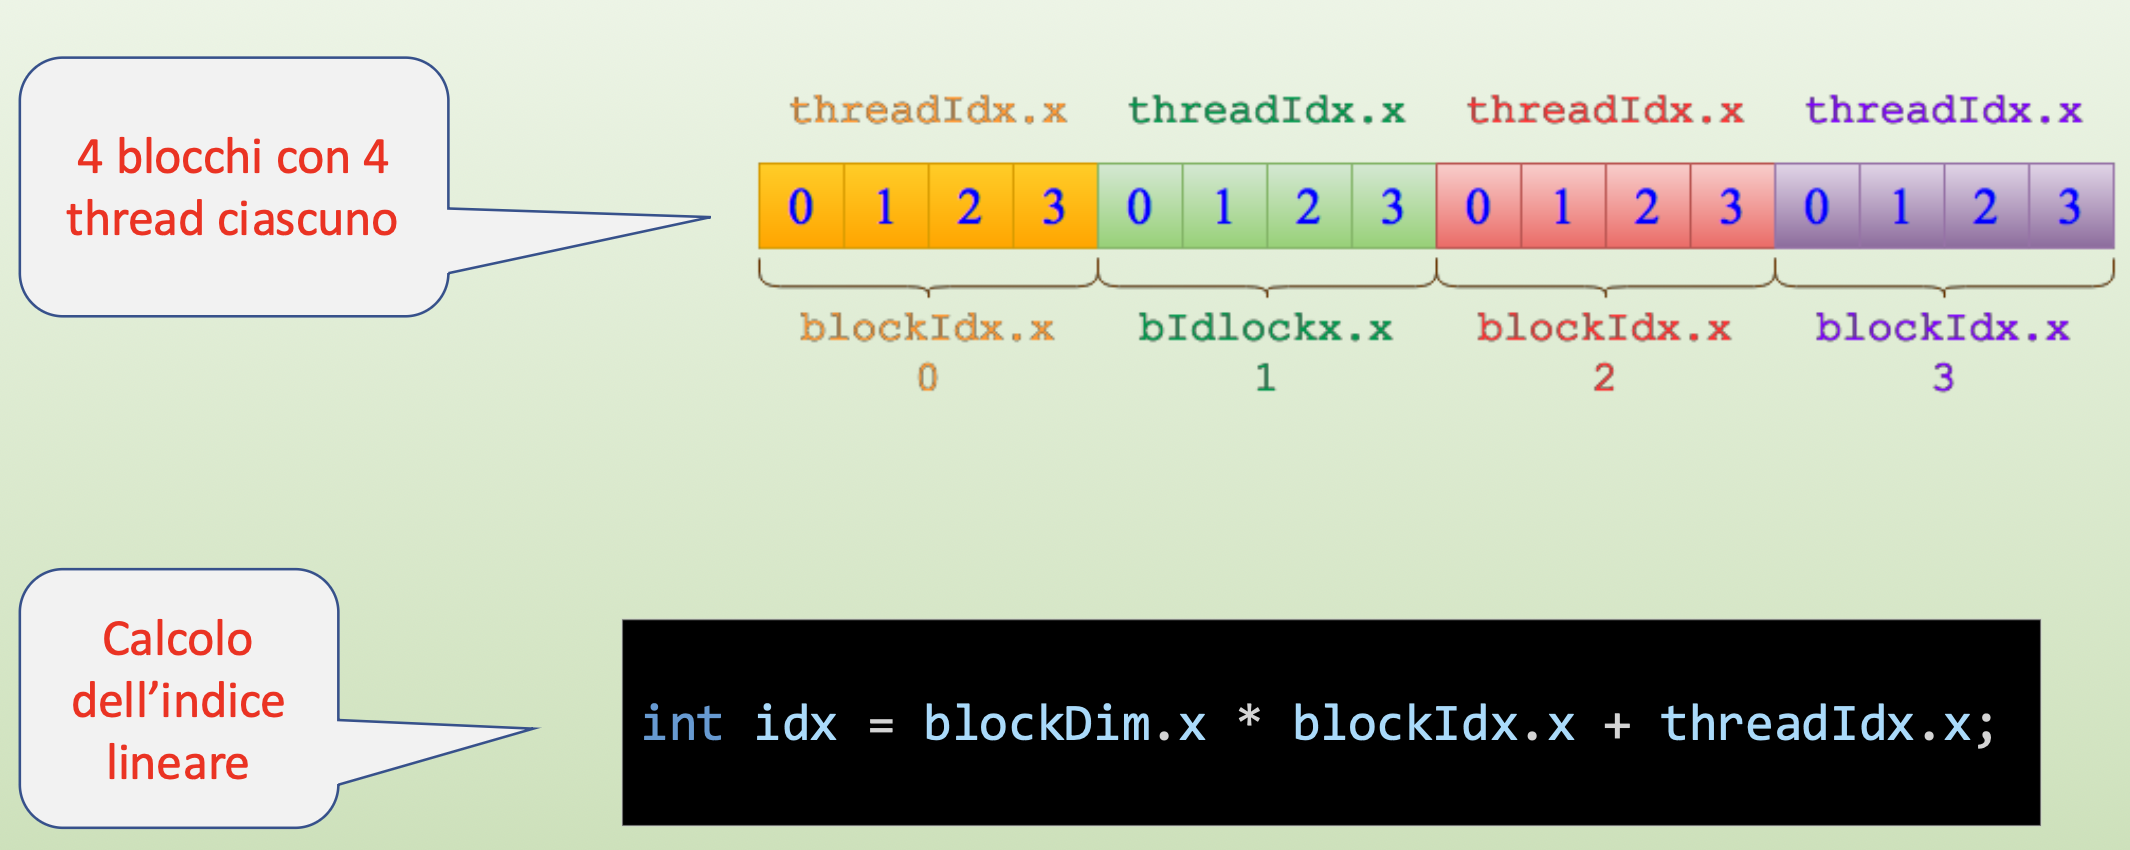
\includegraphics[width=0.8\textwidth]{images/grid1Dcoordinate1D.png}
    \caption{Organizzazione della griglia 1D e coordinate 1D}
\end{figure}

\subsection{Lancio di un kernel CUDA}
Quando prendo una funzione e la lancio con un kernel significa che prendo quella funzione e la lancio sulla GPU, i parametri di configurazione di esecuzione sono fatti in questo modo:
\begin{lstlisting}
    kernel<<<gridDim, blockDim>>>(args...);
\end{lstlisting}
Il primo valore \texttt{gridDim} specifica la dimensione della griglia di blocchi, mentre il secondo valore \texttt{blockDim} specifica la dimensione di ciascun blocco di thread. Gli argomenti \texttt{args...} rappresentano i parametri da passare al kernel.

\subsection{Kernel concorrenti}
Potrebbe verificarsi che numerosi kernel vengano lanciati sullo stesso host (dallo stesso processo o da processi diversi), potrei trovarmi nella situazione in cui ho diversi blocchi concorrenti sullo stesso device.

Esiste l'api \underline{cudaDeviceSynchronize} che permette di sincronizzare l'esecuzione dei kernel, significa che la cpu si sincronizza con tutti i kernel, praticamente il lancio del kernel diventa bloccante.

\subsection{Restrizioni del kernel}
\begin{itemize}
    \item Accede alla memoria globale
    \item Restituisce void
    \item non supporta numero variabile di argomenti, devono essere specificati
    \item non supporta le variabili statiche
    \item ha un comportamento asincrono rispetto al chiamante
\end{itemize}

\subsection{Memoria}
E' praticamente una trasposizione 1 a 1 della memoria in C, le funzioni servono per allocare memoria sul device in global memory (ricordasi che i thread accedono tutti alla global memory):
\begin{itemize}
    \item cudaMalloc: alloca memoria sul device
    \item cudaFree: dealloca memoria sul device
    \item cudaMemcpy: copia dati tra host e device
    \item cudaMemset: imposta un valore nella memoria del device
\end{itemize}
Il trasferimento e l'allocazione di memoria sono operazioni sincrone, l'host si ferma in attesa del completamento di queste operazioni.

cudaMalloc ritorna un doppio puntatore, che e' quello che viene passato ai kernel per puntare correttamente allo spazio di indirizzamento del device (memoria globale), la size e' in byte, il puntatore e' di tipo void\*:
\begin{lstlisting}
    cudaError_t cudaMalloc(void** devPtr, size_t size);
\end{lstlisting}

restituisce un codice di errore. La cudaFree e' quella che libera la memoria.

I puntatori su host e device sono diversi, non e' possibile fare assegnamenti tra uno e l'altro invece bisogna usare la cudaMemcpy.

Non c'e' sempre un mapping 1-1 tra i puntatori host e device, guardiamo ora il mapping tra griglia 2d e coordinate 2d.
Se prendiamo una griglia di blocchi 2x2 mostriamo gli indici dei blocchi e dei thread all'interno, mostriamo che poiche' i tre campi vengono definiti quando definiamo le griglie dobbiamo capire come usare x e y, il campo x viene considerato come campo che varia sulle colonne della matrice per converso la y indica le righe della matrice e si muove in verticale pensando che l'origine e' in alto a sinistra. Posso creare un doppio ordine per x e y di indici e le coppie ordinate mi indicizzano tutte le entry della matrice:

\begin{figure}[ht!]
    \centering
    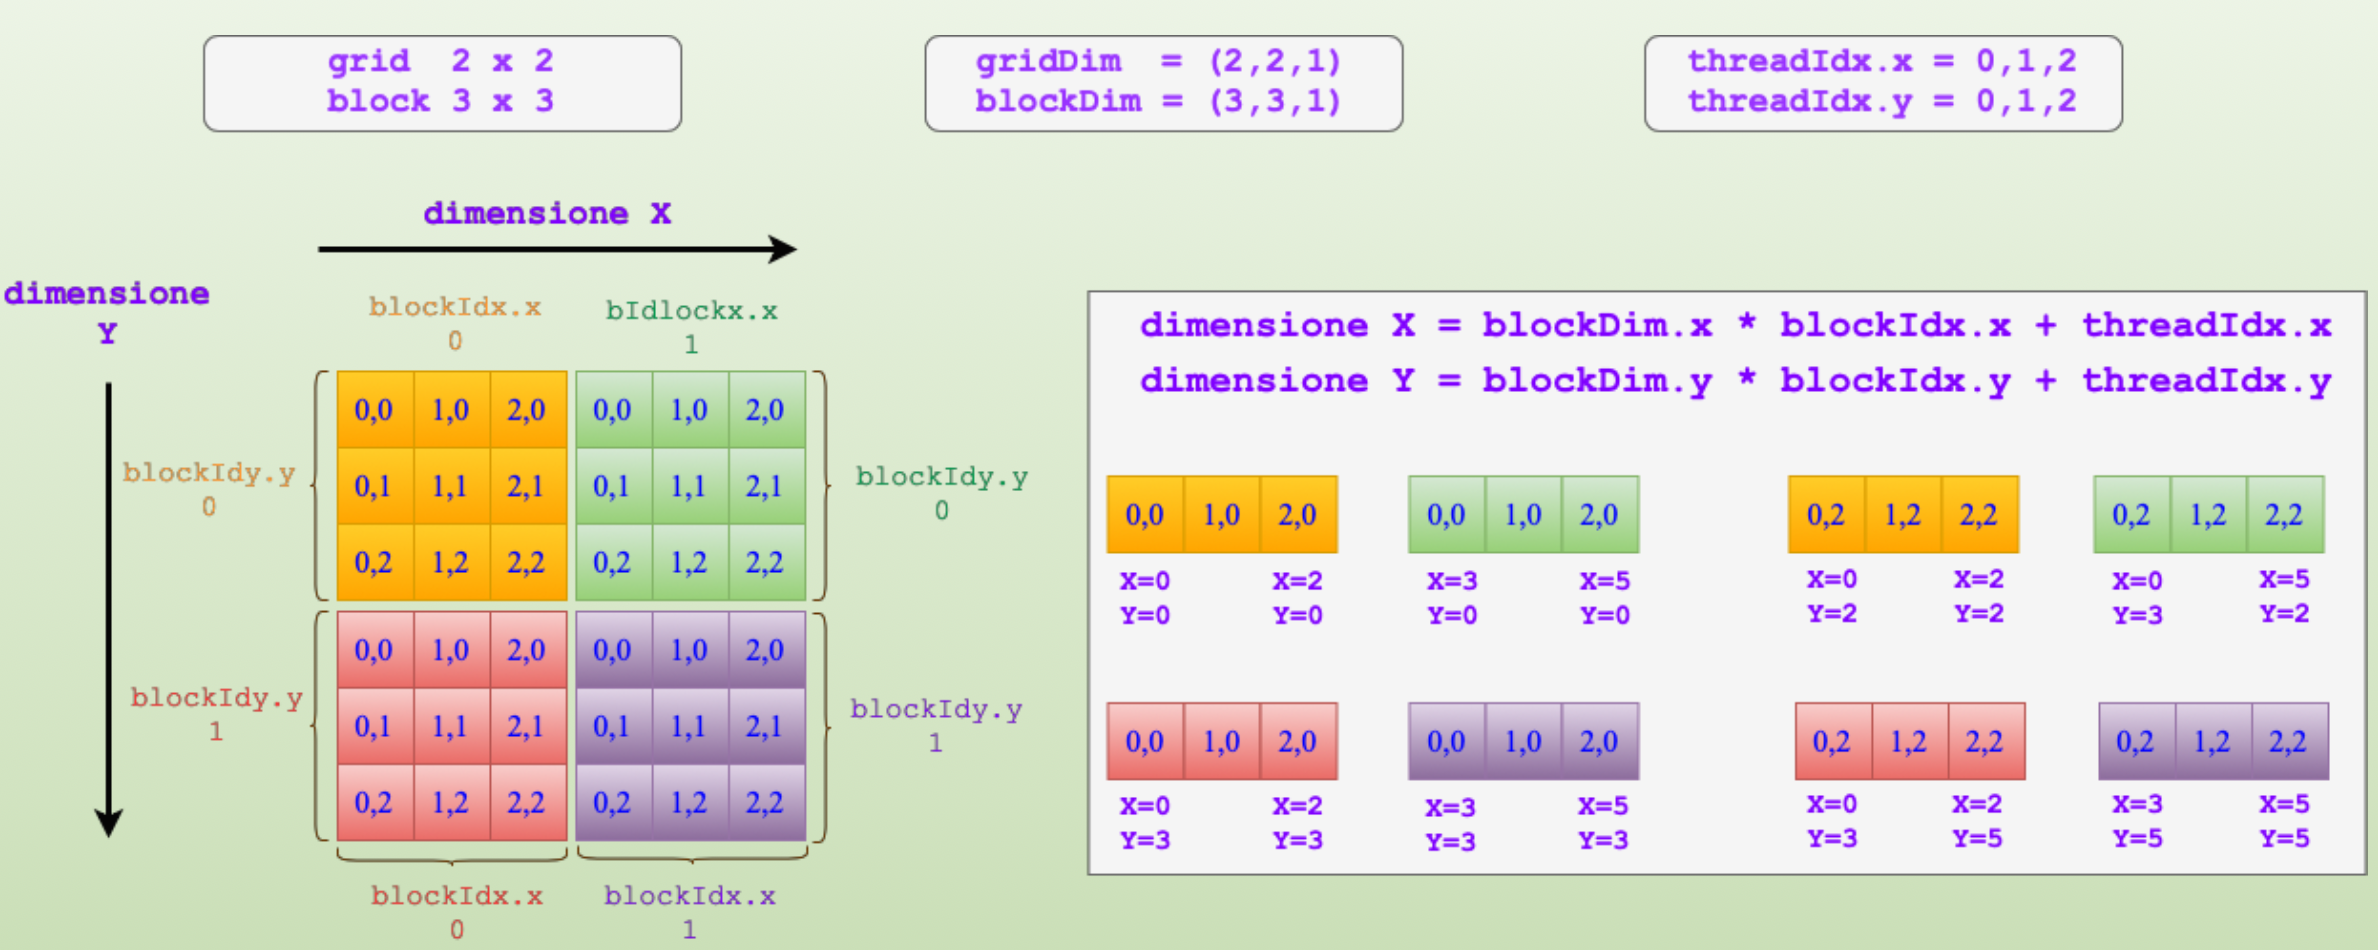
\includegraphics[width=0.8\textwidth]{images/grid2d.png}
\end{figure}

Abbiamo quindi prodotto delle coordinate 2d (x,y) per ogni thread all'interno della griglia 2D e a questo punto e' sufficiente spostarsi nella colonna e nella riga:
\begin{lstlisting}
    int ix = blockDim.x * blockIdx.x + threadIdx.x;
    int iy = blockDim.y * blockIdx.y + threadIdx.y;
\end{lstlisting}
A questo punto l'indice linearizzato lo ricaviamo in questo modo:
\begin{lstlisting}
    int id = iy * nx + ix;
\end{lstlisting}

\begin{figure}[ht!]
    \centering
    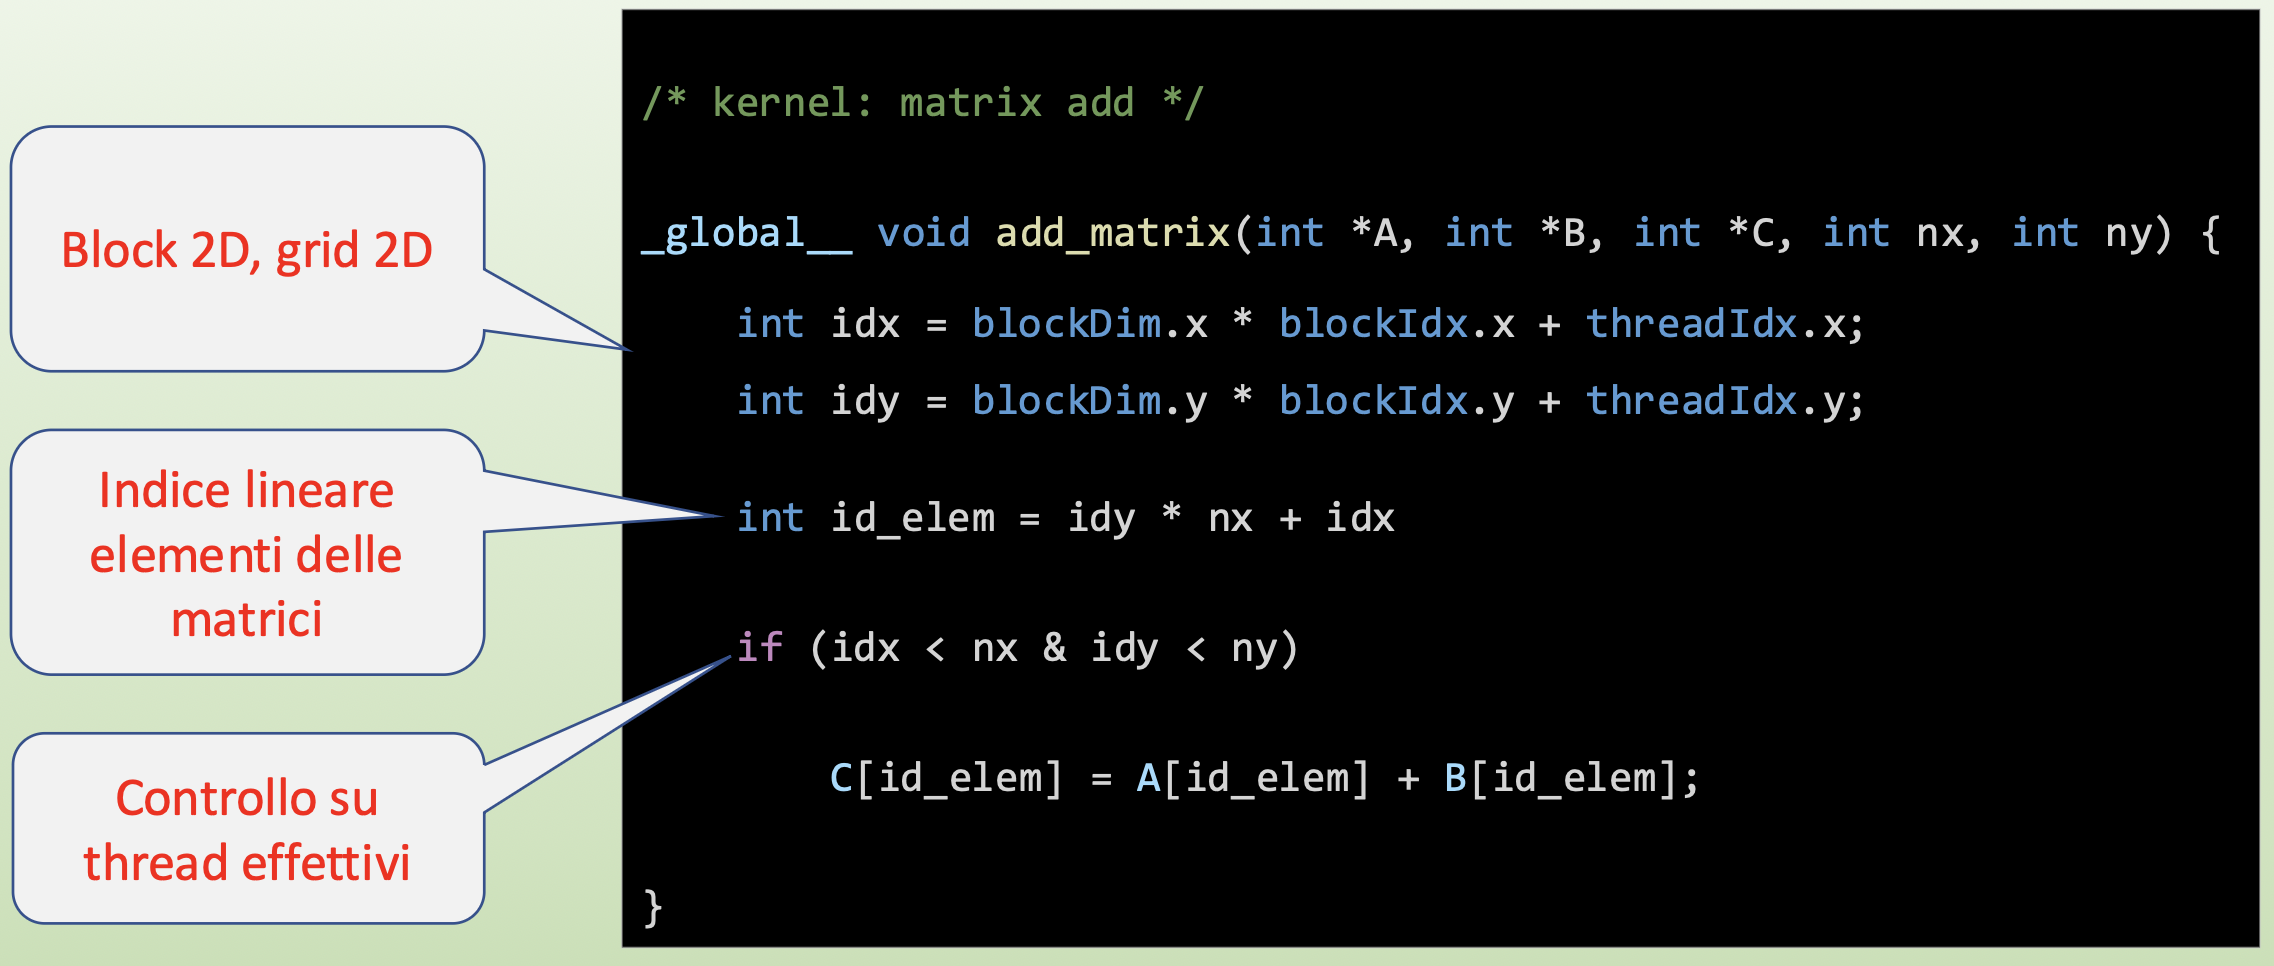
\includegraphics[width=0.8\textwidth]{images/sommaMatriciKernel.png}
\end{figure}

Se si deve trattare una matrice che rappresenta l'immagine, si possono organizzare blocchi di dimensione fissata (16x16) e calcolare la griglia di conseguenza (5x4).

\section{Modello di esecuzione CUDA}
Vogliamo vedere cosa succede a questa miriade di thread che vengono eseguiti nelle GPU, come si arriva ai core. Lo faremo in modo astratto dall'architettura, senza entrare nei dettagli specifici delle implementazioni hardware.

\subsection{Panoramica}

Quando abbiamo un thread che ha le sue risorse private (dei registri assegnati ad uno spazio locale) ed e' a sua volta in grado di chiamare delle funzioni. I thread vengono ordinati in blocchi, il blocco viene attribuito ad uno streaming multi-processor e devono essere eseguiti in parallelo su una risorsa. Vi e' l'uso e lo scambio di memorie veloci, la shared memory per la comunicazione inter-thread. Una griglia (grid) e' un array di thread block che eseguono tutti lo stesso kernel, legge e scrive in global memory e sincronizza le chiamate di kernel tra loro dipendenti.
L'architettura della GPU e' disegnata come un array scalabile di streming multiprocessors, il parallelismo hardware della GPU e' ottenuto replicando questo elemento base.
Gli elementi di uno streaming multiprocessor tipo sono:
\begin{itemize}
    \item CUDA core
    \item Memory: global - shared - texture - constant
    \item caches
    \item registri per la memoria locale
    \item unita' load/store per i/o
    \item unita' per funzioni specializzate, come funzioni algebrice sin, cos, exp
    \item scheduler dei wrap
\end{itemize}
Gli vengono assegnati i blocchi e lui e' in grado di gestire i blocchi attraverso lo scheduler.
%immagine streaming multiprocessor

\subsubsection{Mapping logico - fisico dei thread}
In questo panorama dal punto di vista logico si ha un mapping tra thread e core (ogni thread ha un core) un blocco di thread viene eseguito su un streaming multiprocessor e la griglia viene mappata sul device.

\subsubsection{Esecuzione}
\begin{itemize}
    \item mapping gerarchia thread in gerarchia processori sulla GPU
    \item GPU esegue uno o piu' kernel
    \item streaming multiprocessor gestisce i blocchi di thread
    \item un thread block e' schedulato solo su un SM 
    \item I core eseguono i thread
    \item Gli SM eseguono i thread a gruppi di 32 thread chiamati warp
\end{itemize}

\subsection{Warp: architettura SIMT}
Gli warp sono gruppi di 32 thread (con ID consecutivi) che messi insieme agli altri warp costituiscono un blocco. Ha una semantica che richiama al modello SIMD perche' idealmente si vorrebbe che i thread nel worp eseguissero simultaneamente la stessa istruzione. Questa cosa e' un problema perche' ogni thread ha un flusso a se, quindi si ricorre al modello SIMT questo implica perdita di efficienza. Ogni thread ha il suo program counter e register state. Ogni thread puo' eseguire cammini distinti di esecuzione delle istruzioni. I thread che compongono un warp iniziano assieme allo stesso indirizzo del progamma.
32 e' un numero magico, ha origine dall'HW ed e' fondamentale nella programmazione CUDA per la scalabilita' e trasparenza. E' l'unita' minima di esecuzione che permette grande efficienza nell'uso della GPU. Ha un forte impatto sulle presatzioni degli algoritmi sviluppati. Concettualmente ha un comportamento modello SIMD ma nella pratica assume un modello SIMT.

\subsubsection{HW multi-threading}
Questi sono gli elementi HW di un ambiente multi-threading:
\begin{figure}[ht!]
    \centering
    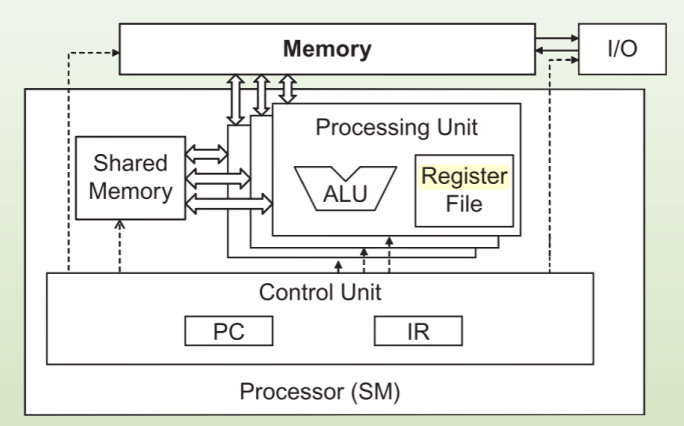
\includegraphics[width=0.8\textwidth]{images/hwMultithreading.png}
\end{figure}

\subsubsection{Registri}
I registri sono usati per le variabili automatiche scalari e le coordinate dei thread:

\begin{lstlisting}
    __global__ void matrix_prod(float *a, float *b, float *c) {
        int Row = blockIdx.y * blockDim.y + threadIdx.y;
        int Col = blockIdx.x * blockDim.x + threadIdx.x;
        if (Row < N && Col < N) {
            float sum = 0.0f;
            for (int k = 0; k < N; k++) {
                sum += a[Row * N + k] * b[k * N + Col];
            }
            c[Row * N + Col] = sum;
        }
    }
\end{lstlisting}

\subsubsection{Logica warp}
Dal punto di vista logico i warp mantiene la consistenza ma il blocco la perde un po', lo vediamo come blocco di thread ma quando viene passato alla macchina e diventa attivo questo viene ripartito in warp (la macchina vede una collezione di 32 thread) e poi lo passano al multiprocessore che si occupa dai warp che gli competono, questo accade indipendentemente dalla dimensione di griglia che abbiamo fissato.
I warp condizionano come noi creiamo il kernel, ad esempio un kernel di 40 blocchi non ha molto senso, dato che dobbiamo eseguire gruppi di 32 thread alla volta e' meglio avere multipli di 32 (gli altri rimarrebbero inattivi e si mangerebbero risorse inutili).
Uno warp puo' essere attivo o disattivo, e' attivo quando le risorse di computazione gli vengono assegnate, quando e' attivo si puo' trovare in diversi stati:
\begin{itemize}
    \item selezionato: in esecuzione su un dato path (preso in carico dallo scheduler di warp)
    \item bloccato: non pronto per l'esecuzione
    \item candidato: eleggibile se tutti e 32 i core sono liberi e tutti gli argomenti della prossima istruzione sono disponibili
\end{itemize}
%formula calcolo warp per blocco

\subsubsection{Scheduling dei blocchi}
Come funziona lo scheduling dei blocchi, ogni streaming multiprocessor riceve un numero di blocchi (questo varia a seconda di quanti SM ho) questo per non lasciare IDLE gli SM.

\subsubsection{Ripartizione risorse}
Le risorse vengono ripartite a seconda della griglia che andiamo a definire e nel momento in cui vengono ripartite non c'e' context switch ed e' per questo che cio' che puo' essere attivo e' limitato.
Esistono limiti imposti dall'HW, come ad esempio il numero di blocchi che possono essere attivi contemporaneamente su un SM, il numero di thread per blocco, il numero di registri per thread, la dimensione della shared memory per blocco, la dimensione della global memory per blocco. 

L'occupancy e' il tasso tra warp attivi e numero massimo di warp per SM:
\[
\text{occupancy} = \frac{\text{warp attivi}}{\text{numero massimo di warp per SM}}
\]

Esiste un flag di uno strumento di profilazione per calcolare l'occupancy:
\begin{lstlisting}
    nvprof --metrics achieved_occupancy ./Application
\end{lstlisting}

\subsection{Latency hiding}
Il grado di parallelismo a livello di thread utile a massimizzare l'utilizzo delle unita' funzionali di un SM dipende dal numero di warp residenti e attivi nel tempo. 
La latenza e' definita come il numero di cicli necessari al completamento dell'istruzione. Per massimizzare il throughput occorre che lo scheduler abia sempre warp eleggibili ad ogni ciclo di clock. Si ha cosi' latency hiding quando i warp in attesa di esecuzione possono essere utilizzati per mascherare la latenza delle operazioni in corso.
Classificazione dei tipi di istruzione che inducono latenza:
\begin{itemize}
    \item Istruzioni aritmetiche: tempo necessario per la terminazione dell'operazione
    \item Istruzioni di memoria: tempo necessario al dato per giungere a destinazione
\end{itemize}

\subsection{Warp divergence}
La divergenza e' un altro nemico insieme alla latenza, si esplicita in modo chiaro, ci sono dei branch all'interno del codice (if else), semplicemente difronte ad un thread si ha un ritardi sistematico e perdiamo la natura del parallelismo di un warp. Fa cadere il modello SIMD e diventa SIMT.

\begin{lstlisting}
    __global__ void pari_dispari_1(int *c) {
        int tid = blockIdx.x * blockDim.x + threadIdx.x;
        int a = 0, b = 0;

        if (tid % 2 == 0) {
            a = 2;
        } else {
            b = 1;
        }

        c[tid] = a + b;
    }
\end{lstlisting}

Il compilatore fa dell'ottimizzazione per la divergenza (dove puo' ovviamente), aggiunge dei predicati alle istruzioni che verificano il vero o falso, calcolano quindi il predicato logico e le istruzioni del predicato e a questo punto i thread calcolano i predicati e non si sequenzializzano.

\begin{lstlisting}
    if (x < 0) {
        z = x - 2
    }
    else if (x >= 0) {
        z = x + 2
    }


    p = (x<0)
    p: z = x - 2
    !p: z = x + 2
\end{lstlisting}

\subsection{Sincronizzazione}
E' un altro aspetto fondamentale a livello di blocco, i thread possono seguire strade diverse e possono avere tempi diversi. Possiamo arrivare ad uno stadio in cui tutti dei thread hanno finito la loro esecuzione, e' importante quindi impostare delle barriere di sincronizzazione in cui tutti i thread si aspettano, questo per evitare delle race condition e per fare in modo di usare il risultato di altri thread.
Si puo' fare a livello di sistema, aspettiamo che venga completato un dato task su entrambi host e divice:
\begin{lstlisting}
    cudaError_t cudaDeviceSynchronize(void);
\end{lstlisting}

ma anche a livello di blocco, si tratta di utilizzare le primitive di sincronizzazione fornite da CUDA, come \texttt{\_\_syncthreads()}, che permette di sincronizzare i thread all'interno di un blocco.
\begin{lstlisting}
    __device__ void __syncthreads(void);
\end{lstlisting}

Ma anche a livello di warp, attendiamo che tutti i thread in un warp raggiungano lo stesso punto di esecuzione:
\begin{lstlisting}
    __device__ void __syncwarp(mask);
\end{lstlisting}

\subsubsection{Deadlock}
Attenzione che sincronizzazione e divergenza possono portare ad un deadlock, quindi è importante progettare attentamente la logica del kernel per evitare situazioni di stallo.
\begin{lstlisting}
    if (threadIdx.x < 16){
        F1();
        __syncthreads();
    }
    else if (threadIdx.x >= 16) {
        F2();
        __syncthreads();
    }
\end{lstlisting}

La prima meta' dei thread aspetta la seconda meta' per completare la propria esecuzione, creando una situazione di stallo.

\subsection{Reduction}
La reduction e' un operazione molto comune che e' la somma degli elementi di array di grandi dimensioni, se lo vogliamo fare in parallelo non e' cosi' scontata, possiamo fare questa cosa quando l'operatore soddisfa le proprieta' commutativa e associativa, questo significa che possiamo fare questa operazione riordinando i dati come vogliamo

Il caso sequenziale e' banale:
\begin{lstlisting}
    float sum = 0.0f;
    for (int i = 0; i < N; i++) {
        sum += array[i];
    }
\end{lstlisting}

Il caso parallelo e' piu' complesso, dobbiamo dividere i dati in parti uguali, ogni thread calcola la somma della sua parte e poi si fa una somma finale. L'idea quindi e' di fare somma parziali memorizzate in-place nel vettore stesso, sommiami gli elementi di un livello sulla meta' degli elementi del livello sottostante, cosi' facendo teniamo un albero di log n (dove n sono i dati che devono essere sommati).
Conviene ricondursi a tecniche ricorsive:
\begin{lstlisting}
    int recursiveReduce(int *data, int const size) {
        //terminazione
        if (size == 1) return data[0];

        //rinnova lo stride
        int const stride = size / 2;

        //riduzione in loco
        for (int i = 0; i < stride; i++) {
            data[i] += data[i + stride];
        }

        //chiamata ricorsiva
        return recursiveReduce(data, stride);
    }
\end{lstlisting}

Da qui possiamo pensare ad una strategia ricorsiva:
\begin{itemize}
    \item Ad ogni passo un numero di thread pari alla meta' degli elementi dell'array effettua le somme parziali nella prima meta' degli elementi, riduzione
    \item il numero di thread attivi si dimezza ad ogni passo rinnovare lo stride
    \item occorre sincronizzare il comportamento dei thread affinche' tutti i thread al passo t abbiano terminato il compito prima di andare al passo successivo t + 1 (analogo alla chiamata ricorsiva)
\end{itemize}

Dobbiamo pensare che i dati li dividiamo in blocchi, e poi combinare i risultati parziali usciti dai blocchi:
\begin{figure}[ht!]
    \centering
    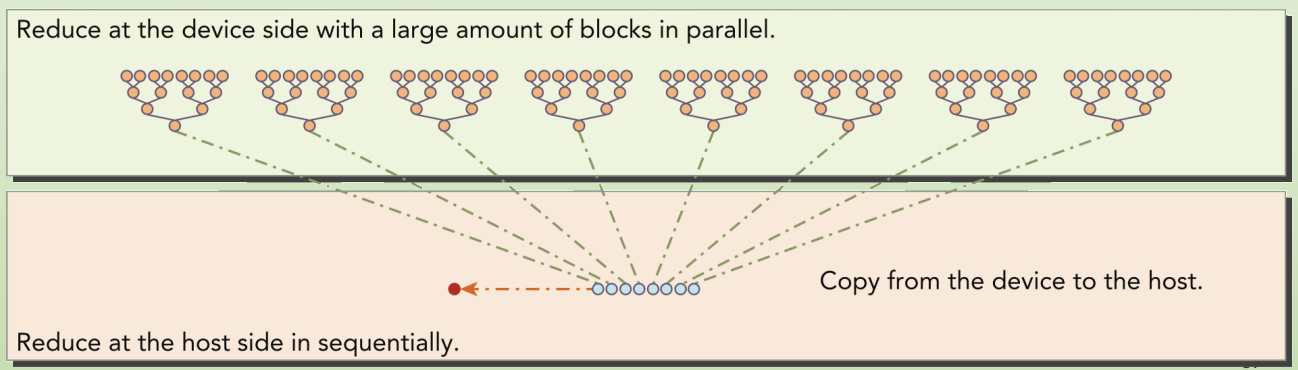
\includegraphics[width=0.8\textwidth]{images/sommeParzialiBlocchi.png}
\end{figure}

%direi che si potrebbe mettere anche il codice della soluzione parallela con la risoluzione della warp divergence

\begin{figure}[ht!]
    \centering
    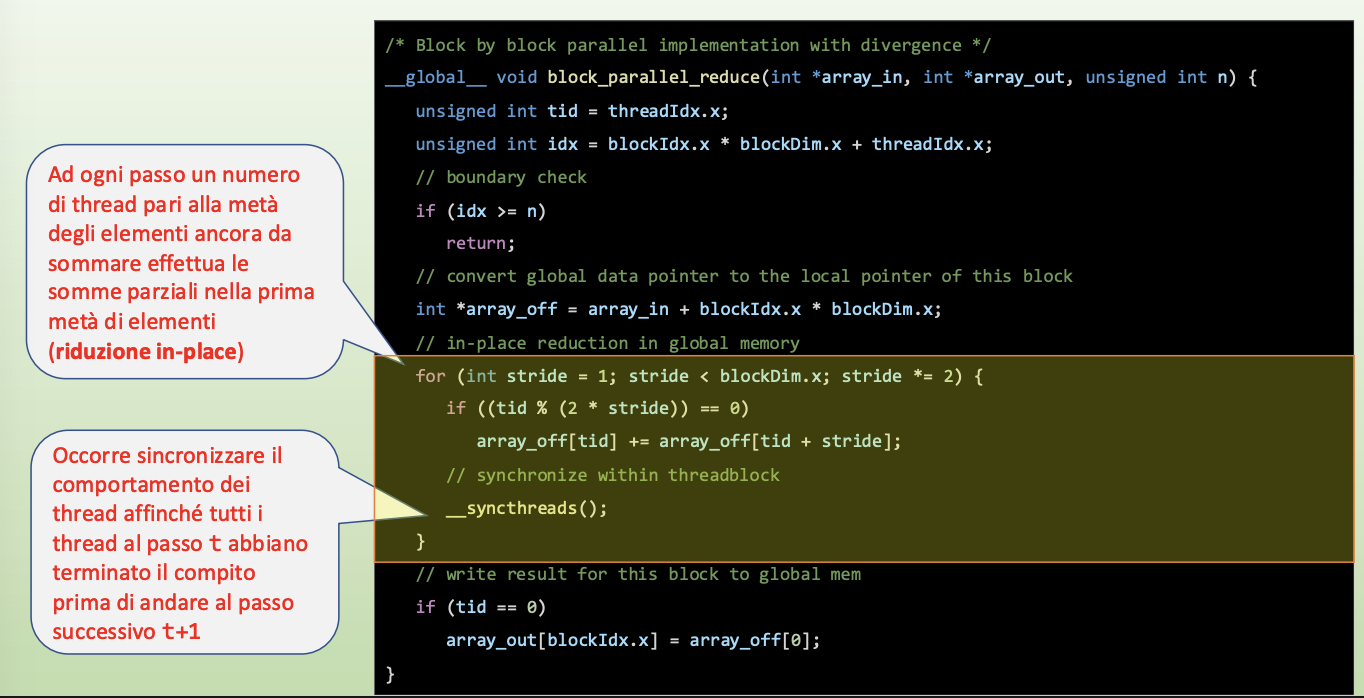
\includegraphics[width=0.8\textwidth]{images/reduction.png}
\end{figure}

Questa soluzione ha il problema della divergenza dei warp, l'if in cui controlliamo che l'indice del thread sia pari, possiamo pero' eliminare l'if:
\begin{lstlisting}
    for (int stride =1; stride < blockDim.x; stride *= 2) {
        //convert tid into local array index 
        int index = 2* stride * tid;
        if(index < blockDim.x) {
            idata[index] += idata[index + stride];
        //synchronize within threadblock
        __syncthreads();
    }
\end{lstlisting}

\subsection{Operazioni atomiche}
Poniamo un problema per porre il pretesto di usare delle operazioni atomiche che di perse' garantiscono l'accesso corretto ed univoco ai dati anche se piu' thread accedono allo stesso dato.
L'istogramma di un immagine e' l'intensita' del colore RGB in un'immagine. Per calcolarlo ci serve avere operazioni atomiche perche' dobbiamo incrementare l'array di intensita' RGB accedendo in modo concorrente agli stessi pixel con piu' thread.

Le operazioni atomiche in CUDA eseguono solo operazioni matematiche ma senza interruzione da parte di altri thread questo perche' sono tradotte in una singola istruzione, sono definite da cuda:
\begin{lstlisting}
    int atomicAdd(int *address, int val);
\end{lstlisting}

Le operazioni basilari sono:
\begin{itemize}
    \item Matematiche: add, subtract, maximum, minimum, increment, decrement
    \item Bitwise: AND, bitwise OR, bitwise XOR
    \item Swap: scambiano valore in moemoria con uno nuovo
\end{itemize}

L'idea per calcolare l'istogramma e' semplice, si alloca una struttura dati (un array lungo 3 * 256) per mantenere i valori dell'istrogramma e , per ogni pixel dell'immagine si effettua una atomicAdd() per incrementare il valore della frequenza dei colori presenti nel pixel.

\begin{lstlisting}
/*
 * Kernel 1D that computes histogram on GPU
 */
__global__ void ppm_histGPU(PPM ppm, int *histogram) {

   uint x = blockIdx.x * blockDim.x + threadIdx.x;

  // pixel out of range
   if (x >= ppm.width * ppm.height)
      return;

   // colors of the pixel
   color R = ppm.image[3 * x];
   color G = ppm.image[3 * x + 1];
   color B = ppm.image[3 * x + 2];

   // use atomic
   atomicAdd(&histogram[R], 1);
   atomicAdd(&histogram[G+256], 1);
   atomicAdd(&histogram[B+512], 1);
}
\end{lstlisting}

\subsubsection{Prodotto matriciale}
Come facciamo ad ottenere il prodotto tra matrici sfruttando la blocchettizzazione. Quello che dobbiamo fare e' definire una griglia definendo il mapping tra indici di thread e delle matrici. Da notare che le dimensioni rilevanti sono 2, numero di righe n della amtrice A e il numero m di colonne della matrice B. 